%Группа 51-1 Модуль 2
\title{Занятие №1}
\begin{listofex}
	\item Какие числа называют простыми? Какие составными?
	\item Выберите из данных числе простые:
	\begin{enumcols}[itemcolumns=10]
		\item \( 4 \)
		\item \( 15 \)
		\item \( 7 \)
		\item \( 17 \)
		\item \( 27 \)
		\item \( 51 \)
		\item \( 37 \)
		\item \( 81 \)
		\item \( 57 \)
		\item \( 67 \)
	\end{enumcols}
	\item Представьте составное число в виде произведения простых:
	\begin{enumcols}[itemcolumns=3]
		\item \( 24 \)
		\item \( 36 \)
		\item \( 30 \)
		\item \( 50 \)
		\item \( 98 \)
		\item \( 288 \)
		\item \( 1000 \)
		\item \( 520 \)
		\item \( 225 \)
	\end{enumcols}
	\item Найдите наибольший общий делитель двух чисел:
	\begin{enumcols}[itemcolumns=4]
		\item НОД\( (30;\;25) \)
		\item НОД\( (24;\;40) \)
		\item НОД\( (60;\;88) \)
		\item НОД\( (81;\;108) \)
		\item НОД\( (24;\;40) \)
		\item НОД\( (20;\;100) \)
		\item НОД\( (23;\;61) \)
		\item НОД\( (4;\;92) \)
	\end{enumcols}
	\item Найдите наибольший общий делитель трех чисел:
	\begin{enumcols}[itemcolumns=2]
		\item НОД\( (66;\;44;\;88) \)
		\item НОД\( (64;\;80;\;44) \)
	\end{enumcols}
	\item Найдите наименьшее общее кратное двух чисел:
	\begin{enumcols}[itemcolumns=4]
		\item НОК\( (30;\;25) \)
		\item НОК\( (24;\;40) \)
		\item НОК\( (60;\;88) \)
		\item НОК\( (20;\;100) \)
	\end{enumcols}
\end{listofex}
\newpage
\title{Занятие №2}
\begin{listofex}
	\item Разделите простые и составные числа на две группы:
	\[ 12,\;13,\;25,\;31,\;261,\;19,\;7,\;61,\;121,\;2,\;39,\;61,\;150 \]
	\item Расположите числа в порядке возрастания:
	\[ 50057,\;507,\;5757,\;77755,\;75057,\;7557,\;55577,\;7057,\;570 \]
	\item Вместо звёздочки подставьте, если возможно, цифру так, чтобы получилось правильное
	неравенство:
	\begin{enumcols}[itemcolumns=3]
		\item \( 3128 < 312\:* \)
		\item \( 5782 > 57*2 \)
		\item \( 38*46 < 38300 \)
	\end{enumcols}
	\item Разложите на простые множители:
	\begin{enumcols}[itemcolumns=4]
		\item \( 84 \)
		\item \( 112 \)
		\item \( 280 \)
		\item \( 4500 \)
	\end{enumcols}
	\item Найдите:
	\begin{enumcols}[itemcolumns=4]
		\item НОД\( (45;\;60) \)
		\item НОД\( (27;\;36) \)
		\item НОД\( (54;\;36) \)
		\item НОД\( (220;\;180) \)
	\end{enumcols}
	\item Найдите:
	\begin{enumcols}[itemcolumns=4]
		\item НОК\( (45;\;60) \)
		\item НОК\( (27;\;36) \)
		\item НОК\( (34;\;51) \)
		\item НОК\( (120;\;150) \)
	\end{enumcols}
	\item Шоколадка стоит \( 35 \) рублей. В воскресенье в супермаркете действует специальное
	предложение: заплатив за две шоколадки, покупатель получает три (одну в подарок). Сколько
	шоколадок можно получить на \( 200 \) рублей в воскресенье?
\end{listofex}
\newpage
\title{Домашняя работа №1}
\begin{listofex}
	\item Найдите:
	\begin{enumcols}[itemcolumns=4]
		\item НОД\( (48;\;72) \)
		\item НОД\( (36;\;42) \)
		\item НОК\( (48;\;72) \)
		\item НОК\( (36;\;42) \)
	\end{enumcols}
\end{listofex}
%\newpage
%\title{Занятие №3}
%\begin{listofex}
%
%\end{listofex}
%\newpage
%\title{Занятие №4}
%\begin{listofex}
%
%\end{listofex}
%\newpage
%\title{Домашняя работа №2}
%\begin{listofex}
%
%\end{listofex}
%\newpage
%\title{Занятие №5}
%\begin{listofex}
%
%\end{listofex}
%\newpage
%\title{Занятие №6}
%\begin{listofex}
%
%\end{listofex}
%\newpage
%\title{Занятие №7}
%\begin{listofex}
%
%\end{listofex}
%\newpage
%\title{Проверочная работа}
%\begin{listofex}
%
%\end{listofex}
\newpage
\title{Консультация}
\begin{listofex}
	\item Сумма пяти различных натуральных (то есть целых положительных) чисел равна 100. Какое
	наибольшее значение может принимать самое больше из этих чисел?
	\item Прямоугольник на рисунке составлен из 7 квадратов. Сторона каждого закрашенного квадрата
	равна 4см. Чему равна сторона большого белого квадрата?
	\begin{center}
		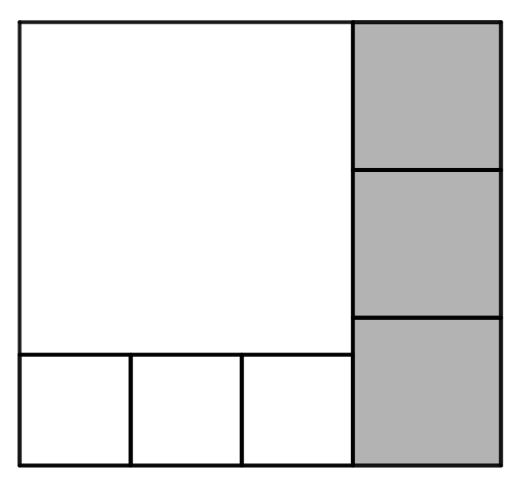
\includegraphics[width=0.3\linewidth]{124.jpg}
	\end{center}
	\item Незнайка хотел купить пять порций мороженого, но ему не хватило 80 рублей. Тогда он купил две порции мороженого, и у него осталось 70 рублей. Сколько денег было у Незнайки изначально?
	\item На доске выписаны в порядке возрастания все пятизначные числа, в записи которых используются
	пять последовательных цифр. Какое число идет после \( 59876 \)?
	\item Малыш, Карлсон и Винни-Пух съели торт. Они ели одновременно и каждый ел торт с одной и
	той же скоростью. Малышу досталась только \( 1/13 \) часть торта. А вот если бы Малыш ел только с Карлсоном, то ему бы досталась четверть торта. Какую долю торта съел бы Малыш, если бы он ел только с Винни-Пухом? (В ответе укажите такое число \( N \), что Малышу достанется \( 1/N \) часть торта)

	\item Решить ребус: ЦВЕТОК \( + \) ЦВЕТОК \( + \) ЦВЕТОК \( = \) БУКЕТИК
\end{listofex}